
\documentclass[border=1pt]{standalone}
\usepackage[T1]{fontenc}
\usepackage{newtxtext}
\usepackage{newtxmath}
\usepackage{amsmath}
\usepackage{tikz}
\usepackage{pgfplots}
\usepgfplotslibrary{groupplots}
\usetikzlibrary{arrows.meta}
\pgfplotsset{compat=1.18}

\definecolor{cclassical}{HTML}{2166ac}
\definecolor{clearned}{HTML}{b2182b}
\definecolor{cproposed}{HTML}{1a9850}
\definecolor{cref}{HTML}{7f7f7f}
\definecolor{clight}{HTML}{67a9cf}
\definecolor{cbandlo}{HTML}{f4a582}
\definecolor{cbandhi}{HTML}{92c5de}

% Figure text is sized for a 252 pt column: axis labels a touch under the
% 8 pt caption size, tick labels one step below that.
\newcommand{\figlab}{\fontsize{7.5}{8.5}\selectfont}
\newcommand{\figtick}{\fontsize{6.5}{7.5}\selectfont}
\newcommand{\fignote}{\fontsize{6}{7}\selectfont}

\pgfplotsset{
  every axis/.append style={
    line width=0.5pt,
    scale only axis,
    tick style={line width=0.4pt, black},
    tick pos=left,
    grid=major,
    grid style={gray!30, line width=0.3pt},
    label style={font=\figlab},
    tick label style={font=\figtick},
    title style={font=\figlab, yshift=-2pt},
    legend cell align=left,
    legend style={
      font=\fignote, draw=black!35, fill=white, fill opacity=0.92,
      text opacity=1, inner sep=1.2pt, row sep=-1.5pt, legend image post style={scale=0.7}},
  },
  every axis plot/.append style={line width=0.7pt, mark size=1.3pt},
}
\begin{document}
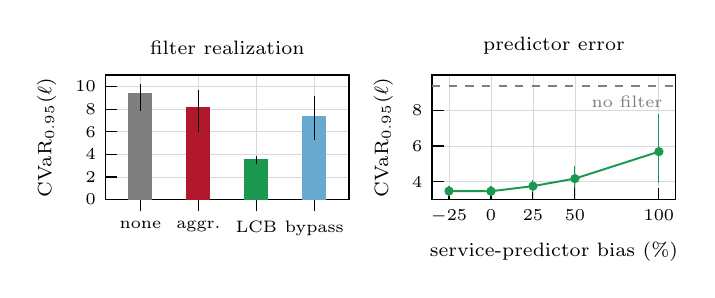
\begin{tikzpicture}
\begin{groupplot}[
  group style={group size=2 by 1, horizontal sep=30pt},
  width=88pt, height=45pt, ylabel={$\mathrm{CVaR}_{0.95}(\ell)$}]
\nextgroupplot[title={filter realization}, ybar, bar width=8pt, xmin=-0.6, xmax=3.6, ymin=0, ymax=11, xtick={0,1,2,3}, xticklabels={none,aggr.,LCB,bypass}, xticklabel style={font=\fignote}, ytick={0,2,4,6,8,10}]
\addplot[fill=cref, draw=cref, bar shift=0pt, error bars/.cd, y dir=both, y explicit, error bar style={line width=0.4pt, black}, error mark options={line width=0.4pt, mark size=1pt, black}]
  table[x=x, y=y, y error plus=ep, y error minus=em] {
x y ep em
0 9.35982 0.640181 1.28036
};
\addplot[fill=clearned, draw=clearned, bar shift=0pt, error bars/.cd, y dir=both, y explicit, error bar style={line width=0.4pt, black}, error mark options={line width=0.4pt, mark size=1pt, black}]
  table[x=x, y=y, y error plus=ep, y error minus=em] {
x y ep em
1 8.09487 1.31365 1.90513
};
\addplot[fill=cproposed, draw=cproposed, bar shift=0pt, error bars/.cd, y dir=both, y explicit, error bar style={line width=0.4pt, black}, error mark options={line width=0.4pt, mark size=1pt, black}]
  table[x=x, y=y, y error plus=ep, y error minus=em] {
x y ep em
2 3.46829 0.13912 0.118183
};
\addplot[fill=clight, draw=clight, bar shift=0pt, error bars/.cd, y dir=both, y explicit, error bar style={line width=0.4pt, black}, error mark options={line width=0.4pt, mark size=1pt, black}]
  table[x=x, y=y, y error plus=ep, y error minus=em] {
x y ep em
3 7.28003 1.61938 1.73507
};
\nextgroupplot[title={predictor error}, xmin=-35, xmax=110, ymin=3.0, ymax=9.95982, xtick={-25,0,25,50,100}, xlabel={service-predictor bias (\%)}]
\addplot[cproposed, mark=*, error bars/.cd, y dir=both, y explicit,
  error bar style={line width=0.4pt}, error mark options={line width=0.4pt, mark size=1pt}]
  table[x=x, y=y, y error plus=ep, y error minus=em] {
x y ep em
-25 3.4793 0.112524 0.0978101
0 3.46829 0.13912 0.118183
25 3.75461 0.193709 0.186736
50 4.17429 0.575773 0.387335
100 5.68186 1.92523 1.58483
};

\addplot[cref, dashed, line width=0.6pt, forget plot] coordinates {(-35,9.35982) (110,9.35982)};
\node[font=\fignote, text=cref, anchor=north east] at (axis cs:108,9.35982) {no filter};
\end{groupplot}
\end{tikzpicture}
\end{document}
